
\section{Processing system}

As discussed in the previous chapter processing system of the library relies on components.
Core of the library is responsible just for creating component graph.
The processing of \lsystem and producing results is fully under control of component graph.
This gives absolute freedom to user in implementing process system.

However it is hard to design and implement whole \lsystem processing system from scratch.
Library contains rich set of predefined components from which can be assembled many different component graphs.
The predefined components have general interface which allows user to reuse or extend them to add new functionality with minimum of effort.



\subsection{Basic component system}

Component system designed in this section are primarily used for processing \lsystems to produce 2D and 3D graphics in the web interface.
However component system is designed to be extensible to any output type.

\lsystems are generally processed in two phases.
First phase is rewriting where axiom (initial string of symbols) is rewritten by rewrite rules and second phase is interpreting result string of symbols.
This can be done with two components, the Rewriter which is responsible for rewriting the \lsystem to given iteration and the Interpreter which is responsible for interpreting symbols and producing output (\autoref{fig:simpleSystem}).

\begin{figure}[h!]
	\centering
	\begin{tikzpicture}[->,auto,node distance=3cm,>=latex,shorten >=2pt]
		\node (in) [coord] {};
		\node (rw) [block, right of=in] {Rewriter};
		\node (int) [block, right=1cm of rw] {Interpreter};
		\node (out) [coord, right of=int] {};
		
		\draw (in) -- node {input} (rw);
		\draw (rw) -- (int);
		\draw (int) -- node {output} (out);
	\end{tikzpicture}
	\caption{Simple \lsystem processing system}
	\label{fig:simpleSystem}
\end{figure}

However components in the system in \autoref{fig:simpleSystem} have too much tasks to do thus they will be complicated to implement and hard to extend and test.

System in \autoref{fig:advancedSystem} was created by subdivision of previous system.
The Rewriter component was split to the Rewriter and the Iterator.
The Rewriter will do just rewriting of given symbols and the Iterator will control iterating of \lsystem (repetitive rewriting).
The Interpreter component was split to the Interpreter and the Renderer.
The Interpreter will do interpreting of symbols which means keep position of virtual turtle in space, saving and loading of states etc.
The Renderer will just produce the output.
If we need to create different output type we have to implement only new renderer component and rest of the system will remain unchanged.

\begin{figure}[h!]
	\centering
	\begin{tikzpicture}[->,auto,node distance=3cm,>=latex,shorten >=2pt]
		\node (rw) [block] {Rewriter};
		\node (iter) [block, right of=rw] {Iterator};
		\node (in) [coord, above of=iter, node distance=15mm] {};
		\node (inter) [block, right of=iter] {Interpreter};
		\node (rend) [block, right of=inter] {Renderer};
		\node (out) [coord, right of=rend] {};
		
		\draw (rw) to[bend left=40] (iter);
		\draw (iter) to[bend left=40] (rw);
		\draw (in) -- node {input} (iter);
		\draw (iter) -- (inter);
		\draw (inter) -- (rend);
		\draw (rend) -- node {output} (out);
	\end{tikzpicture}
	\caption{Subdivided \lsystem processing system}
	\label{fig:advancedSystem}
\end{figure}


\subsection{Component system extensions}
\label{sec:caller}

The system in \autoref{fig:callerComponent} can be enhanced even more.
Every interpreter needs to translate symbols to interpretation methods itself which can be done by specialized component called \emph{Interpreter caller}.
This component can be smart enough to explore all components in the system, find all interpretation methods and do translation automatically.
This causes automatic connection of all interpreters to interpreter caller.
More interpreters can be used with advantage for example for processing \lsystems which interacts with self or their Environment \cite{MP96}.
One interpreter actual model ant the second interprets environment.

\begin{figure}[h!]
	\centering
	\begin{tikzpicture}[->,auto,node distance=3cm,>=latex,shorten >=2pt]
		\node (iter) [block] {Iterator};
		\node (in) [coord, above of=iter, node distance=15mm] {};
		\node (rw) [block, below of=iter, node distance=20mm] {Rewriter};
		\node (caller) [blockx, right of=iter, node distance=35mm] {Interpreter caller};
		\node (inter) [block, right of=caller, node distance=40mm] {Interpreter};
		\node (env) [block, below of=inter, node distance=20mm] {Environment module};
		\node (rend) [block, right of=inter] {Renderer};
		\node (out) [coord, right of=rend] {};
		
		\draw (rw) to[bend left=40] (iter);
		\draw (iter) to[bend left=40] (rw);
		\draw (in) -- node {input} (iter);
		\draw (iter) -- (caller);
		\draw [dashed] (caller) -- (inter);
		\draw [dashed] (caller) -- (env);
		\draw (inter) -- (rend);
		\draw (env) -- (rw);
		\draw (rend) -- node {output} (out);
	\end{tikzpicture}
	\caption{Advantage of Interpreter caller component which can automatically call more interpreters}
	\label{fig:callerComponent}
\end{figure}




Next necessary component is called \emph{Random provider}.
It provides controlled behavior for random number generation described in \autoref{sec:measuring}.
This component provides function which returns random number and can be called by other components or by user in \lsystem definition.
This component is connected to iterator to correctly reset random seed every pass.

\emph{Axiom provider} is next extending component and it provides axiom to the Iterator.
Axiom provider is wrapper around single symbol property called axiom.
The Iterator is designed generally to take axiom from any component implementing \texttt{ISymbolProvider} so it is possible to connect for example another Rewriter as axiom provider (\autoref{fig:inputProvider}).

\begin{figure}[h!]
	\centering
	\begin{tikzpicture}[->,auto,node distance=3cm,>=latex,shorten >=2pt]
		\node (iter) [block] {Iterator};
		\node (rw) [block, left of=iter] {Main rewriter};
		\node (rw2) [blockx, above of=iter, node distance=20mm] {Input rewriter};
		\node (in) [coord, above of=rw2, node distance=15mm] {};
		\node (caller) [block, right of=iter, node distance=35mm] {Interpreter caller};
		\node (inter) [block, above of=caller, node distance=20mm] {Interpreter};
		\node (rend) [block, right of=inter] {Renderer};
		\node (out) [coord, right of=rend] {};
		
		\draw (rw) to[bend left=40] (iter);
		\draw (iter) to[bend left=40] (rw);
		\draw (rw2) -- (iter);
		\draw (in) -- node {input} (rw2);
		\draw (iter) -- (caller);
		\draw [dashed] (caller) -- (inter);
		\draw (inter) -- (rend);
		\draw (rend) -- node {output} (out);
	\end{tikzpicture}
	\caption{Input of iterator can be supplied by another component}
	\label{fig:inputProvider}
\end{figure}



\subsection{Interpretation of symbol as another \lsystem}
\label{sec:innerLsystem}

In some situations it can be handy to interpret symbol as another \lsystem.
Component system of the library is very versatile and it allows to create specialized component which will be responsible for that.

The component is called \emph{Inner \lsystem processor}.
It is connected to the Interpreter caller and when the caller needs to interpret symbol as \lsystem it will call the Inner \lsystem processor which take care of it.
Component graph with Inner \lsystem processor component is shown in \autoref{fig:innerSystem}.

The Inner \lsystem processor internally works in similar way how the Process manager do (see \autoref{sec:inputProcessing}).
For every processed symbol it builds new components graph for processing inner \lsystem.
The components graph can be specified by special process configuration which needs to be defined in the input\footnote{
	The only implementation of Inner \lsystem processor the \hyperref[Malsys.Processing.Components.Common.ILsystemInLsystemProcessor]{\emph{ILsystemInLsystemProcessor}} component
		uses process configuration called \emph{InnerLsystemConfig} for creating inner component graph.
	This process configuration must be defined (see the definition in the Standard library \ref{sec:innerLsystemConfig}).}.
Interpreter caller in inner component graph is automatically connected to all interpreters in original component graph (see \autoref{sec:caller}) therefore inner \lsystem is interpreted by the same interpreter as the main \lsystem.
Inner interpreter caller is also connected to the Inner \lsystem processor thus it is possible to interpret symbol as another \lsystem even in inner \lsystem.

The creation of inner component graph is relatively complex operation but the created and used component graphs are cached and reused later.

\begin{figure}[h!]
	\centering
	\begin{tikzpicture}[->,auto,node distance=3cm,>=latex,shorten >=2pt]
		\node (it) [block] {Iterator};
		\node (in) [coord, above of=it, node distance=15mm] {};
		\node (rw) [block, left of=it] {Rewriter};
		\node (caller) [block, right of=it, node distance=35mm] {Interpreter caller};
		\node (inter) [block, above of=caller, node distance=20mm] {Interpreter};
		\node (rend) [block, right of=inter] {Renderer};
		\node (out) [coord, right of=rend] {};
		\node (inner) [blockx, below of=caller, node distance=20mm] {Inner L-system processor};
		\node (innerIt) [blockx, below of=inner, node distance=22mm] {Inner iterator};
		\node (innerRw) [blockx, left of=innerIt, node distance=33mm] {Inner rewriter};
		\node (innerCaller) [blockx, right of=innerIt, node distance=32mm] {Inner caller};
		
		\node (innerArea) [area,fit=(innerIt) (innerRw) (innerCaller), label=above left:Inner component graph] {};
		
		\draw (rw) to[bend left=40] (it);
		\draw (it) to[bend left=40] (rw);
		\draw (in) -- node {input} (it);
		\draw (it) -- (caller);
		\draw (caller) -- (inner);
		\draw [dashed] (caller) -- (inter);
		\draw (inter) -- (rend);
		\draw (rend) -- node {output} (out);
		
		\draw [snakeline] (inner) -- (innerArea);
		\draw (innerRw) to[bend left=20] (innerIt);
		\draw (innerIt) to[bend left=20] (innerRw);
		\draw (innerIt) -- (innerCaller);
		\draw (innerCaller) -- (inner);
		\draw [dashed] (innerCaller) to[bend right] (inter);
	\end{tikzpicture}
	\caption{Component system for interpretation symbol as another \lsystem}
	\label{fig:innerSystem}
\end{figure}

Interpretation of symbol as another \lsystem is demonstrated in \autoref{fig:innerLsystem}.
The Pythagoras tree is made of Menger sponges.
Number of iterations of each Menger sponges depends on its size.
The smallest Menger sponges (zero iteration) have extra blossom as demonstration of interpretation symbol as \lsystem in inner \lsystem.
The iteration of the Blossom determines number of leafs and it is randomly selected from 4 to 6.


\begin{figure}[p]
	\centering
	\subfloat[4th iteration]{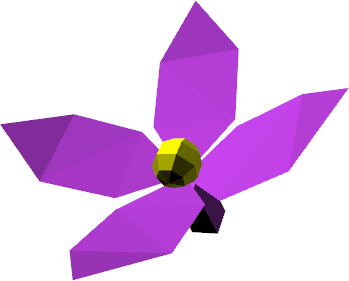
\includegraphics[scale=0.3]{Bloom4}}
	\subfloat[5th iteration]{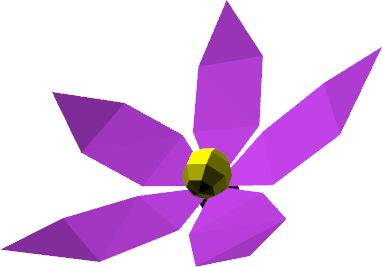
\includegraphics[scale=0.3]{Bloom5}}
	\subfloat[6th iteration]{
\includegraphics[scale=0.3]{Bloom6}}
	\\
	\subfloat[11th iteration of Pythagoras tree]{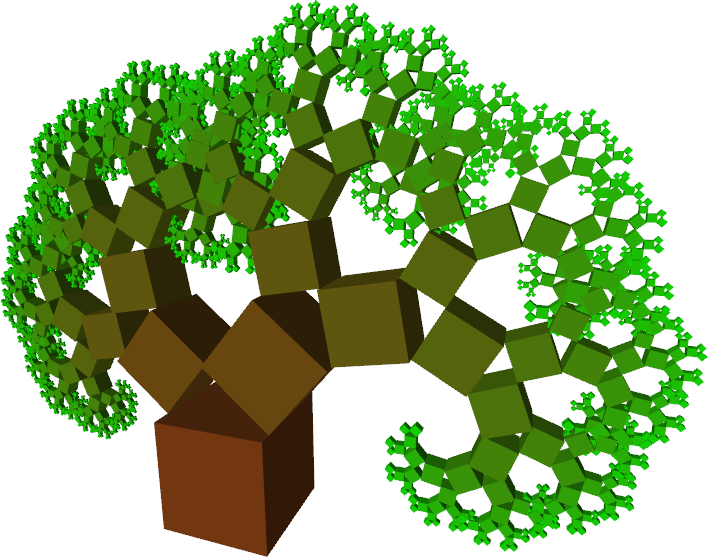
\includegraphics[width=0.55\textwidth]{Pythagoras}} ~
	\subfloat[3rd iteration of Menger sponge]{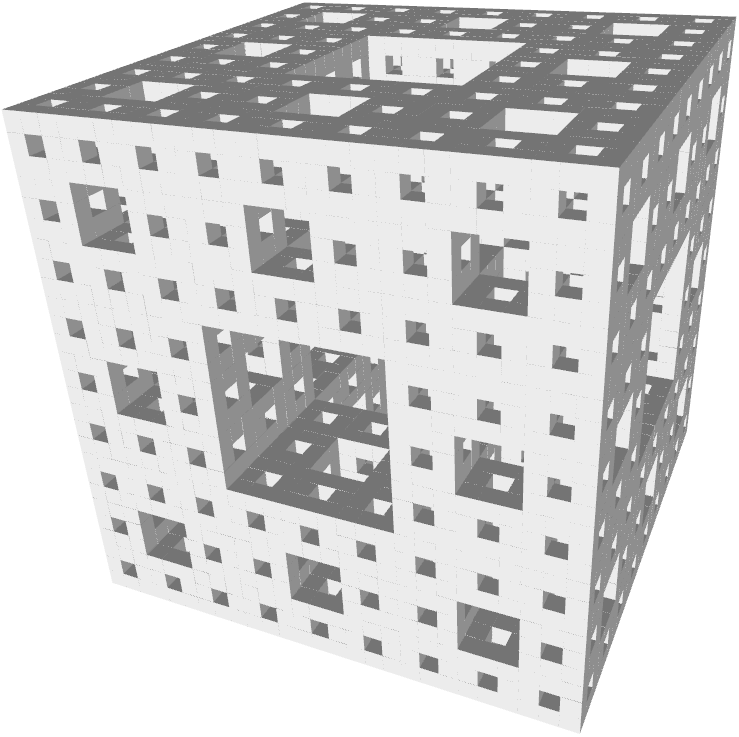
\includegraphics[width=0.40\textwidth]{MengerSponge}}
	\\
	\subfloat[Pythagoras tree made of Menger sponges with blossoms at the smallest cubes]{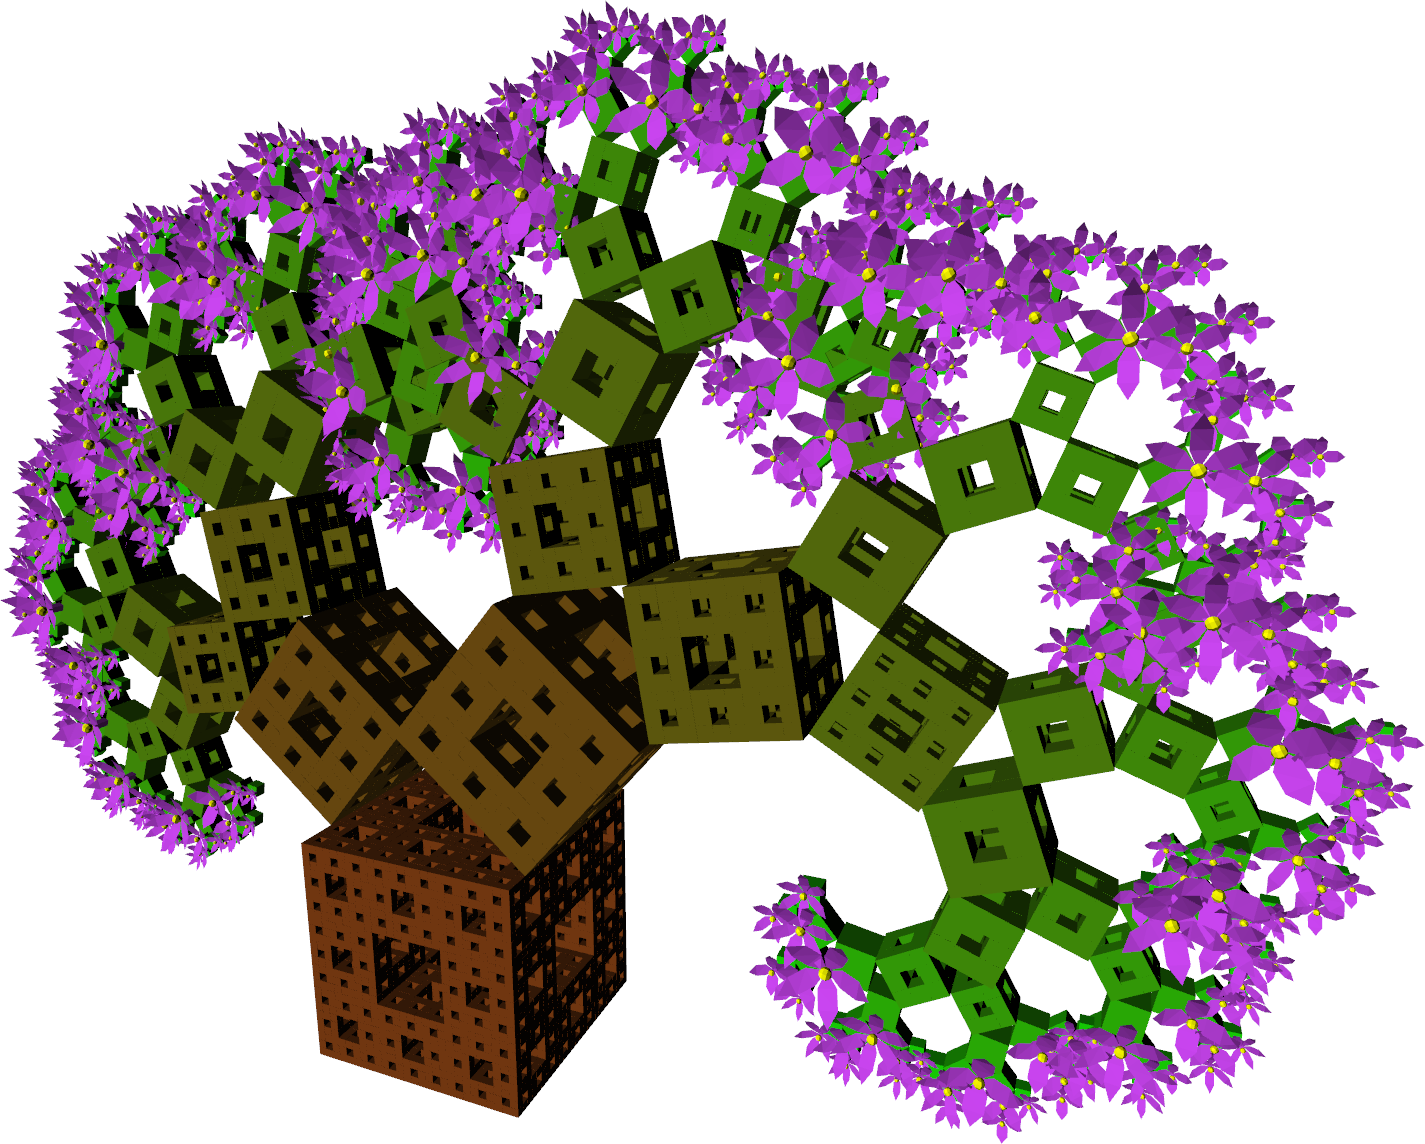
\includegraphics[width=0.9\textwidth]{HybridPythagoras}\label{fig:innerLsystemResult}}
	\caption{Example of interpreting symbol as another \lsystem}
	\label{fig:innerLsystem}
\end{figure}

\begin{Lsystem}[label=lsys:innerLsystem,caption={Source code of \lsystem (\autoref{fig:innerLsystemResult}) demonstrating usage of interpreting symbol as another \lsystem}]
lsystem HybridPythagorasTree(angle = 50) extends Branches {
	let angleComp = 90 - angle;  // angle complement
	let sinAngle = sin(deg2rad(angle));
	let sinAngleComp = sin(deg2rad(angleComp));
	set iterations = 8;
	set symbols axiom = F(64, 0);
	// interpret E(x) as DrawForward(x, x);  // cube
	@interpret E(x) as lsystem MengerSponge(x);@  // Menger sponge
	interpret m as MoveForward;
	interpret + as Yaw(angle);
	interpret - as Yaw(-angleComp);
	rewrite F(x)
		with left = x * sinAngle, right = x * sinAngleComp
		to E(x) [ + m(left / 2) F(right) ] - m(right / 2) F(left);
}

lsystem MengerSponge(size = 1) extends StdLsystem3D {
	let iters = if(size > 50, 2, if(size > 10, 1, 0));
	let cubeSize = size * (1/3)^iters;
	let renderBlooms = iters == 0;
	// add iteration to render blooms
	let iters = iters + if(renderBlooms, 1, 0);
	set iterations = iters;
	set symbols axiom = F;
	interpret F as DrawForward(cubeSize, cubeSize, #EEEEEE);
	interpret f as MoveForward(cubeSize / 2);
	@interpret B as lsystem Bloom(cubeSize);@  // renderes bloom
	rewrite F where renderBlooms to F [ ^ f B ];
	rewrite F to - f f + & f f ^ F F F +f+f- F F +f+f- F F +f+f- F
		-f+f+f^f F F &f&f^ F F &f&f^ F ^ ^ f f f & + f F F &f&f^ F
		^ ^ f f f & + f F F &f&f^ F ^ ^ f f f & + f F f & f f ^ +
		+ f f - f f f f f;
	rewrite f to f f f;
}

lsystem Bloom(size = 1) extends Polygons {
	let color = #d649ff;
	let leafCount = floor(random(4, 7));
	let angle = 150 / leafCount;
	set iterations = leafCount;
	set symbols axiom = F [ G(size/8) K ] leaf;
	interpret F as DrawForward(size * 0.5, size * 0.2, color);
	interpret G as MoveForward(size * 0.5);
	interpret K as DrawSphere(size / 6, #FFFF00);
	interpret + as Yaw(angle);
	interpret - as Yaw(-angle);
	interpret / as Roll;
	interpret ^ as Pitch(-15);
	rewrite leaf to /(360 / leafCount) [ ^(90) <(color) .
		+ ^ G . - ^ G . - ^ G . + +(180) + G . - ^ G .  > ] leaf;
}

process HybridPythagorasTree with ThreeJsRenderer;
\end{Lsystem}



\subsection{Final component system}

Final component system uses all described functionality.
Component graph is shown in \autoref{fig:finalSystem}.
Two main \emph{process configurations} defined in the standard library uses this scheme, namely the \hyperref[configurationSvgRenderer]{\emph{SvgRenderer}} and the \hyperref[configurationThreeJsRenderer]{\emph{ThreeJsRenderer}}
	(see appendix \ref{sec:stdLibProcessConfigurations}).

\begin{figure}[h!]
	\centering
	\begin{tikzpicture}[->,auto, node distance=3cm,>=latex,shorten >=2pt]
		\node (it) [block] {Iterator};
		\node (in) [block, above of=it, node distance=20mm] {Axiom provider};
		\node (rand) [block, below left of=it, node distance=28.284mm] {Random generator provider};
		\node (rw) [block, left of=it] {Rewriter};
		\node (caller) [block, right of=it, node distance=35mm] {Interpreter caller};
		\node (inter) [block, above of=caller, node distance=20mm] {Interpreter};
		\node (rend) [block, right of=inter] {Renderer};
		\node (out) [coord, right of=rend] {};
		\node (inner) [block, below of=caller, node distance=20mm] {Inner L-system processor};
				
		\draw (rw) to[bend left=40] (it);
		\draw (it) to[bend left=40] (rw);
		\draw (in) -- (it);
		\draw (it) -- (caller);
		\draw (it) -- (rand);
		\draw (caller) -- (inner);
		\draw [dashed] (caller) -- (inter);
		\draw (inter) -- (rend);
		\draw (rend) -- node {output} (out);
	\end{tikzpicture}
	\caption{Final component system}
	\label{fig:finalSystem}
\end{figure}























